\graphicspath{{img/capture_baryons/}}
%%%%%%%%%%%%%%%%%%%%%%%%%%%%%%%%%%%%%%%%%%%%%%%%%%%%%%%%%%%%%%%%%%%%%
%%%%%%%%%%%%%%%%%%%%%%%%%%%%%%%%%%%%%%%%%%%%%%%%%%%%%%%%%%%%%%%%%%%%%
%%%%%%%%%%%%%%%%%%%%%%%%%%%%%%%%%%%%%%%%%%%%%%%%%%%%%%%%%%%%%%%%%%%%%
\chapter{Dark Matter Capture from Baryonic Matter in Neutron Stars}
\label{chapter:capture_baryons}

\begin{synopsis}
   This chapter is based on the papers~\cite{Bell:2020obw_sep_NucleonStructureStrong,Anzuini:2021lnv_nov_Improvedtreatmentdark}, where we incorporate two important effects that are important when considering dark matter capture from baryons in neutron stars. 
   % Up to this point, all the results presented have assumed that the DM is scattering off point-like particles that are treated as a free Fermi gas. 
   As the momentum transfers involved in the scattering events leading to capture are large, one must account for the internal structure of the baryon. In addition, the high densities of neutron star matter require us to take into account the strong interactions experienced amongst the baryons. We discuss how to properly incorporate both of these effects into the capture formalism presented in this thesis in a self-consistent manner, and discuss their effects on the capture and interaction rates as well as on the threshold cross-sections that a future NS observation would be sensitive to. 
\end{synopsis}
%%%%%%%%%%%%%%%%%%%%%%%%%%%%%%%%%%%%%%%%%%%%%%%%%%%%%%%%%%%%%%%%%%%%%
%%%%%%%%%%%%%%%%%%%%%%%%%%%%%%%%%%%%%%%%%%%%%%%%%%%%%%%%%%%%%%%%%%%%%
%%%%%%%%%%%%%%%%%%%%%%%%%%%%%%%%%%%%%%%%%%%%%%%%%%%%%%%%%%%%%%%%%%%%%

%%%%%%%%%%%%%%%%%%%%%%%%%%%%%%%%%%%%%%%%%%%%%%%%%%%%%%%%%%%%%%%%%%%%%
%%%%%%%%%%%%%%%%%%%%%%%%%%%%%%%%%%%%%%%%%%%%%%%%%%%%%%%%%%%%%%%%%%%%%
\section{Baryon Structure and Strong Interactions}
\label{ch5:sec:baryons_in_NSs}
%%%%%%%%%%%%%%%%%%%%%%%%%%%%%%%%%%%%%%%%%%%%%%%%%%%%%%%%%%%%%%%%%%%%%
%%%%%%%%%%%%%%%%%%%%%%%%%%%%%%%%%%%%%%%%%%%%%%%%%%%%%%%%%%%%%%%%%%%%%

%%%%%%%%%%%%%%%%%%%%%%%%%%%%%%%%%%%%%%%%%%%%%%%%%%%%%%%%%%%%%%%%%%%%%
\subsection{Baryon Strong Interactions and Effective Masses}
\label{ch5:subsec:strong_ints_meffs}
%%%%%%%%%%%%%%%%%%%%%%%%%%%%%%%%%%%%%%%%%%%%%%%%%%%%%%%%%%%%%%%%%%%%%

At the extremely high densities found in the interiors of neutron stars, the strong interactions amongst the baryons render the free Fermi gas approximation used in Chapter~\ref{chapter:capture_intro} to model the scattering targets invalid. To account for these interactions in a self-consistent way, they should be included in the Lagrangian used to model the nucleon-rich matter. This is often achieved by including effective Skyrme forces, or through a relativistic mean field theory.

The QMC EoS, described in Section~\ref{ch2:subsec:NS_EoS}, adopts the latter approach. The forces mediated by the Lorentz scalars induce an effective mass for the baryons different from their vacuum value, such that $\mbeff \leq \mi$. In this model, the single particle energy for a baryon with momentum $\vec{p}_i$ can be expressed as
\begin{equation}
   \Ei(p_i) = \sqrt{p_i^2 + [\mbeff(n_b)]^2} + U_i(n_b),
   \label{ch5:eq:}
\end{equation}
where $U_i(n_b)$ is the potential induced by the Lorentz vector forces, which depends on the baryon number density. This expression resembles the dispersion relation for a particle of mass $\mbeff$ under the influence of an external force with corresponding potential $U_i$. Hence, the single-particle energy spectrum of the interacting baryons must be expressed in terms of $\mbeff$ rather than the mass in vacuum, and it is this mass that will enter into the kinematics of the scattering processes.  

Accounting for the strong interactions in this way leads to several modifications to the results obtained in Chapter~\ref{chapter:capture_intro}. Firstly, all appearances of the bare mass $\mi$ are replaced by $\mbeff$ in all the results. This will lead to non-trivial modifications of the capture and interaction rates throughout the star as the mass of the target will decrease deeper into the star (see right panels of Fig.~\ref{ch2:fig:QMC_profiles}).

In addition, the Fermi energies, $\kinFi = \muFi - \mi$, are now calculated according to 
\begin{equation}
   \kinFi(r) = \sqrt{[p_{F,i}(n_i)]^2 + [\mbeff(r)]^2} - \mbeff(r),
   \label{ch5:eq:kinFe_meff}
\end{equation}
where $p_{F,i}$ is the Fermi momentum of species $i$. This becomes the input to the Fermi-Dirac distributions for the capture and interaction rates. In doing this, the number density evaluated in the free Fermi gas apprioximation, Eq.~\ref{ch3:eq:n_free_Fermi}, becomes equal to the true number density, $n_i(r)$, provided by solving the EoS alongside the TOV equations. To see this, substitute Eq.~\ref{ch5:eq:kinFe_meff} into Eq.~\ref{ch3:eq:n_free_Fermi} and make the replacement $\mi\rightarrow \mbeff$ to gets
\begin{align}
   n_\mathrm{free}(\kinFi(r), \mbeff(r)) & = \frac{1}{3\pi^2}\left[ \kinFi(r)(2\mbeff + \kinFi(r))\right]^{3/2}\\
   & = \frac{(p_{F,i}(r)^2 + [\mbeff]^2)^{3/2}}{3\pi^2}\\
   & = \frac{p_{F, i}^3}{3\pi^2}\\
   & = n_i(r)
\end{align}
for a Fermi gas, interacting or otherwise. 
As such, the correction factor used to correct for usign realistic profiles for the target is now $\zeta(r) = 1$.


%%%%%%%%%%%%%%%%%%%%%%%%%%%%%%%%%%
\begin{figure}[t!bp]
   \centering
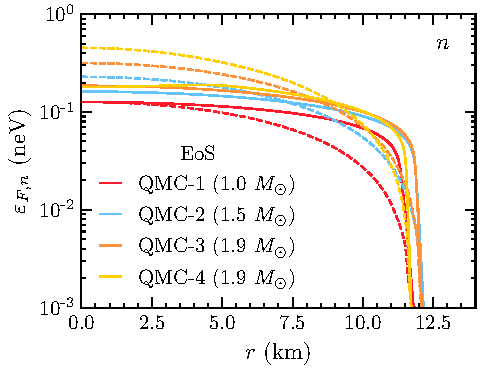
\includegraphics[width=0.495\textwidth]{capture_3/muFn_meff_r_QMC.pdf}
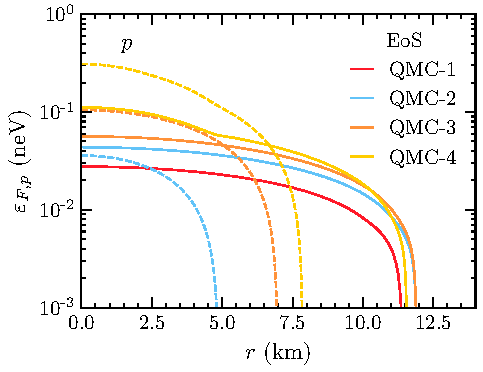
\includegraphics[width=0.495\textwidth]{capture_3/muFp_meff_r_QMC.pdf}
   \caption{Radial profiles of the Fermi energy for neutrons (left) and protons (right). Results are shown for the free Fermi gas (dashed) and interacting baryon (solid) approaches, for the benchmark NS configurations of Table~\ref{ch2:tab:QMC_configs}.
   }
   \label{ch5:fig:muradprofs}
\end{figure}
%%%%%%%%%%%%%%%%%%%%%%%%%%%%%%%%%

In Fig.~\ref{ch5:fig:muradprofs} we show the values of the Fermi energies for neutrons (left panel) and protons (right panel). The dashed lines are the radial profiles used in the free Fermi gas approximation and the solid lines correspond to the calculation outlined above for the effective mass approach. We immediately notice that the profiles for the free Fermi gas approximation are steeper, having larger values in the core and decreasing more rapidly towards the surface, while those obtained with the effective mass approach are quite flat, especially in the core, and go to zero only very close to the surface.

The difference between these two calculations is significantly more prominent for protons. Specifically, in the free Fermi gas approach, we find that protons are non-degenerate in the outer regions of the core and, for light NS configurations such as QMC-1, are non-degenerate throughout the whole star.\footnote{Not shown in Fig.~\ref{ch5:fig:muradprofs} because of the logarithmic scale.}
In contrast, protons are degenerate throughout the entire star in the interacting baryon treatment. 
As we shall see, these different Fermi energies will have important consequences when calculating DM capture and interaction rates, especially for proton targets.


%%%%%%%%%%%%%%%%%%%%%%%%%%%%%%%%%%%%%%%%%%%%%%%%%%%%%%%%%%%%%%%%%%%%%
\subsection{Momentum Dependence of Hadronic Form Factors}
\label{ch5:subsec:mom_dep_FF}
%%%%%%%%%%%%%%%%%%%%%%%%%%%%%%%%%%%%%%%%%%%%%%%%%%%%%%%%%%%%%%%%%%%%%

In the preceeding chapters, we had regarded the target as a point-like particle that the DM scattered off, which is perfectly valid for the leptonic species. Baryons on the other hand are composite particles, being composed of three valence quarks and hence having a finite size. When the momentum transfer exceeds the inverse Compton wavelength of the baryon, $\sim 1/\lambda_\mathcal{B} \sim m_\mathcal{B}$, the internal strucyre begins to be probed, and we must account for their finite size.

As discussed in Section.~\ref{ch1:subsec:quark_to_nucleon_EFT}, this is achieved by reintroducing the momentum dependence in the hadronic form factors, 
\begin{align}
   c_\mathcal{B}^I(t)  &= c_\mathcal{B}^{I}(0) F^2(t),\quad I\in\{S, P, V, A, T\},\\
   F(t) & = \frac{1}{(1 - t/Q_0^2)^2},
\end{align}
where $t$ is the Mandelstam variable, $Q_0$ is an energy scale taken to be $0.9\GeV$, and $c_\mathcal{B}^I(0)$ are the form factors evaluated at zero momentum transfer, with their values given in Appendix~\ref{app:hadronic_matrix_elements}. This factor is included in the matrix elements of the operators in Table.~\ref{ch1:tab:opers_defn_full}, and as such modifies the analytic result for the interaction rate derived in Section~\ref{ch3:sec:diff_int_rate} for matrix elements $\Msq \propto t^n s^m$ to become
\begin{equation}
   \begin{split}
       \Gamma^{-}(E_\chi) & \propto \frac{(-1)^n }{128\pi^3 E_\chi k }\int_0^{E_\chi -m_\chi} dq_0\int \, dt_E \frac{ t_E^n}{(t_E + q_0^2)^{m+\frac{1}{2}}}\frac{1}{(1 + t_E/Q_0^2)^4}\\
       &\hspace{4em}\times\sum_{r=0}^m \mathcal{V}_{m,r}\sum_{j = 0}^r\binom{r}{j} \kinFi^{r-j}  \frac{(-1)^{j} q_0^{j+1}}{j+1} h_j\left( \frac{\Ei^{t^-} - \kinFi}{q_0}\right),
   \end{split}
   \label{ch5:eq:gammaFFfinaltext}
\end{equation}
where $E_i^{t^-}$ and $h_j(x)$ are given in Eqs.~\ref{ch3:eq:Etm_def} and~\ref{ch3:eq:h_stepfn} respectively.

The main effect of these form factors is the suppression of high momentum transfer interactions. This will also increase the DM mass range over which Pauli blocking is expected to be active. We can see these effects by examining the kinematically allowed regions of phase space together with the differential interaction rate profiles.


%%%%%%%%%%%%%%%%%%%%%%%%%%%%%%%%%%%%
\begin{figure}[t!bp] 
   \centering
   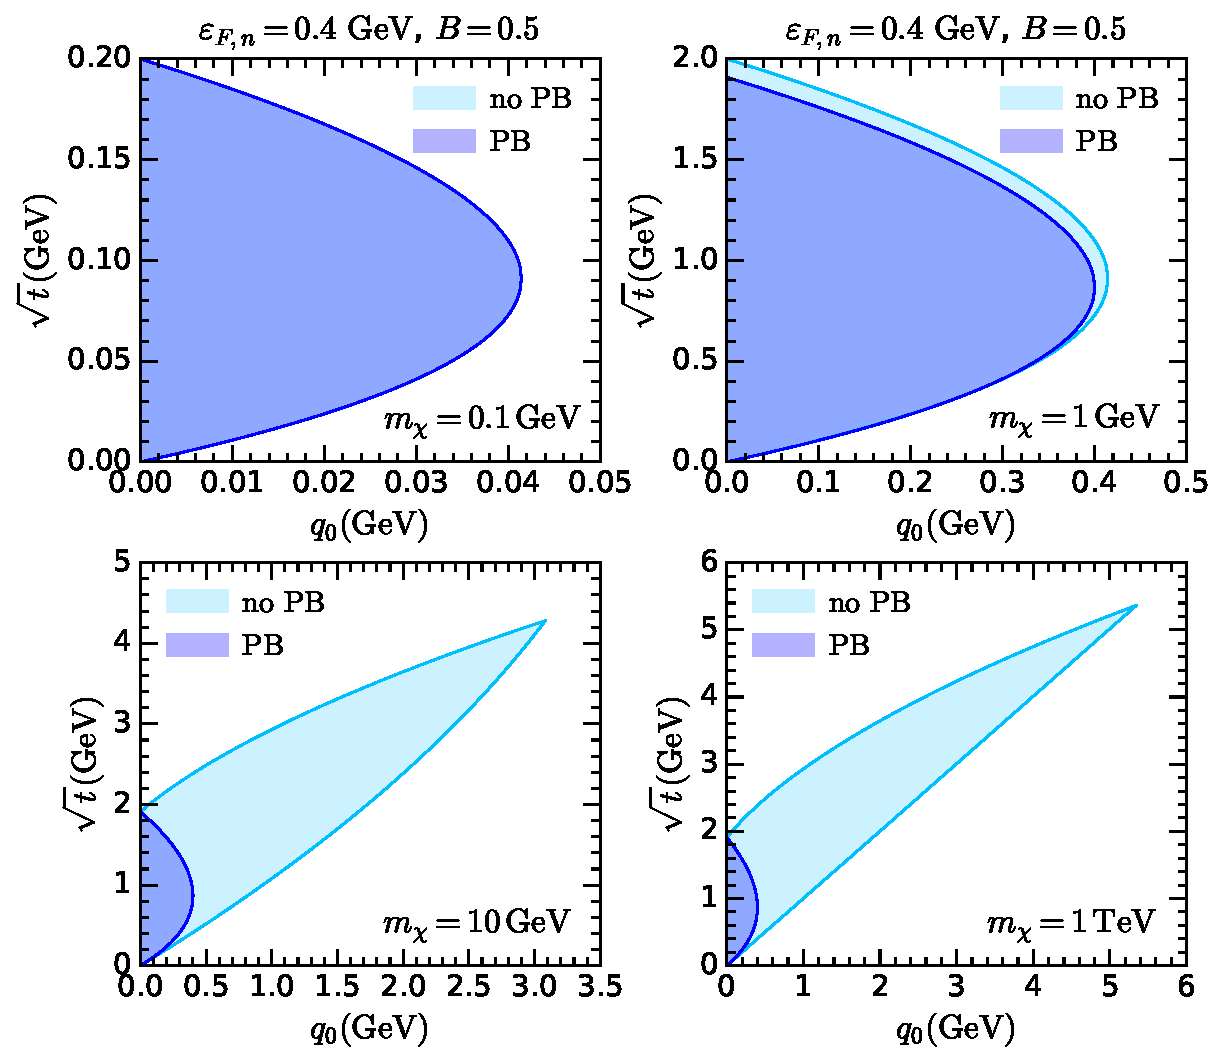
\includegraphics[width=0.75\textwidth]{capture_3/C_int_domain_mdm.pdf}
   \caption{Integration domain for the interaction rate, for different choices of DM mass, assuming   
     $B=0.5$ and $\kinFn=0.4\GeV$. The kinematically allowed region is shaded in light blue and the Pauli suppressed region (PB) in dark blue. 
   }
   \label{ch5:fig:intC}
   \end{figure}
   %%%%%%%%%%%%%%%%%%%%%%%%%%%%%%%%%%%%
   
   
In Fig.~\ref{ch5:fig:intC}, we show how Pauli blocking affects the integration domain of Eq.~\ref{ch5:eq:gammaFFfinaltext}, which is controlled by the smoothed step function $h_0(x)$, for some representative choices of DM mass and the benchmark values $\kinFn=0.4\GeV$ and $B=0.5$.  The region where $h_0(x)=0$ is not kinematically allowed and hence not shown in Fig.~\ref{ch5:fig:intC}.
The light blue area represents the region that is not affected by Pauli blocking (PB), i.e. $h_0(x)=-x$, while the dark blue shaded area indicates the PB region, where $h_0(x)=1$. 
We observe that for light DM masses such as  $m_\chi=0.1\GeV$ (top left panel), the whole domain lies in the PB region. For $m_\chi=1\GeV$ (top right panel), there is a tiny slice of the domain that is not Pauli suppressed. The picture changes dramatically when the DM mass is increased to $m_\chi=10\GeV$ (bottom left panel), where almost the whole integration domain is unaffected by PB. Increasing the DM mass even further, e.g., up to $m_\chi=1\TeV$ (bottom right panel) does not result in much further change to the shape of the domain, demonstrating that the transition between the PB and non-PB regimes occurs between $m_\chi\sim1\GeV$ and $m_\chi\sim10\GeV$.
   


%%%%%%%%%%%%%%%%%%%%%%%%%%%%%%%%%%%%%%%%%%%
\begin{figure}[t!bp] 
\centering
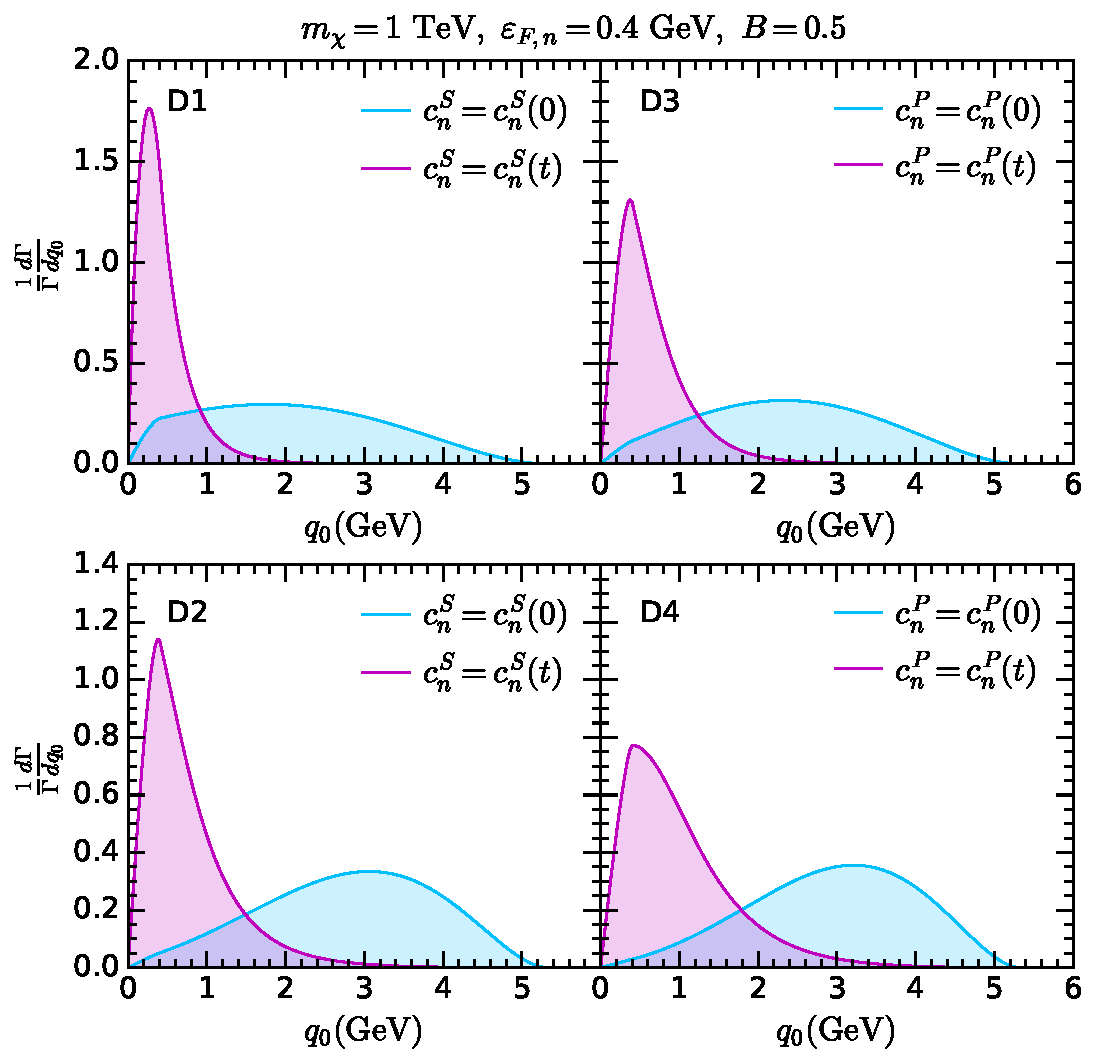
\includegraphics[width=0.95\textwidth]{capture_3/norm_diff_intrate_q_D1-D4.pdf} 
\caption{Normalised differential DM-neutron interaction rate as a function of the DM energy loss, $q_0$, for the operators D1 (top left), D3 (top right), D2 (bottom left) and D4 (bottom right). The light blue lines denote the interaction rate calculated using constant neutron form factors $c_n^S(0)$, $c_n^P(0)$, while the orange lines correspond to that for momentum-dependent couplings $c_n^S(t)$, $c_n^P(t)$. We have set $m_\chi=1\TeV$, $B=0.5$, $\kinFn=0.4\GeV$.
}
\label{ch5:fig:intrateqtr1}
\end{figure}
%%%%%%%%%%%%%%%%%%%%%%%%%%%%%%%%%%%%%%%%%%%



In Fig.~\ref{ch5:fig:intrateqtr1} we show the normalised differential interaction rates for operators D1-D4 as a function of the energy loss $q_0$, calculated with (orange) and without (light blue) momentum dependent couplings, for neutron targets and $m_\chi=1\TeV$. In all cases, we observe that the inclusion of $t$-dependent hadronic matrix elements shifts the peak of the spectrum towards lower energy transfers, $q_0$. 
Thus, the inclusion of $c_i^I(t)$ in Eq.~\ref{ch5:eq:gammaFFfinaltext} suppresses DM-neutron interactions at large momentum transfers. 
Replacing the target mass with the corresponding effective mass $\mbeff\leq m_i$ also shifts the average energy transfer to lower energies.  When both effects are present, a lighter target mass reduces the suppression arising from $t$-dependent form factors. 

%%%%%%%%%%%%%%%%%%%%%%%%%%%%%%%%%%%%%%%%%%%%%%%%%%%%%%%%%%%%%%%%%%%%%
\subsubsection{Asside: Deep Inelastic Scattering}
\label{ch5:subsubsec:DIS}
%%%%%%%%%%%%%%%%%%%%%%%%%%%%%%%%%%%%%%%%%%%%%%%%%%%%%%%%%%%%%%%%%%%%%
Given that the momentum transfer in the DM-nucleon scattering process is sufficiently large that we cannot treat the nucleons as point particles (up to $\sim 10\GeV$ in the cores of the heaviest NSs), one may wonder if there are sizable contributions from Deep Inelastic Scattering (DIS). To that end, we examine the contribution from DIS to the total DM-neutron scattering cross-section. 

The kinematics of DIS of dark matter in NSs is not similar to any case that has previously been treated in the literature, at least not to our knowledge. In contrast to DIS of neutrinos and boosted DM, we are interested in much larger DM masses and relatively lower energies.  Specifically, $E_\chi/m_\chi=1/\sqrt{B}$, where $B$ is the time component of the Schwarzchild metric, which falls in the range $[\sim0.2,\sim0.75]$.  Therefore, we have  $E_\chi\lesssim 2m_\chi$. Following ref.~\cite{Agashe:2014yua_Directdetectionboosted}, we derive the DIS cross-section in NSs for the operators in Table~\ref{ch1:tab:opers_defn_full}. 

The parton level differential cross-section is given by
\begin{equation}
    \frac{d\hat{\sigma}}{d\hat{t}} = \frac{\hat{s}}{8\pi\hat{\gamma}^2}\frac{\hat{s}-(m_\chi^2+x^2m_n^2)}{\hat{s}^2-(m_\chi^2-x^2m_n^2)^2}|\overline{\mathcal{M}}(\hat{s},\hat{t},m_i=x m_n)|^2,
\end{equation}
where $\hat{\gamma} = \gamma(\hat{s}, m_\chi, xm_n)$, $\hat{t}=-Q^2$ is the squared 4-momentum transfer,  $\hat{s} = (1-x)(m_\chi^2-x m_n^2) +xs$, $\Msq$ is defined at the parton level with couplings $g_i=g_q$, and $x$ is the fraction of the nucleon momentum ($P$) carried by the parton, $p=xP$. We define $y$, the fractional energy lost by the DM in the nucleon rest frame~\cite{Agashe:2014yua_Directdetectionboosted}
\begin{equation}
    y = \frac{2q\cdot P}{2k\cdot P} = \frac{-\hat{t}}{\hat{s}-m_\chi^2-x^2m_n^2}, 
\end{equation}
and obtain
\begin{equation}
    dQ^2 = (\hat{s}-m_\chi^2 - x^2m_n^2)dy = x(s - m_\chi^2 - m_n^2)dy. 
\end{equation}
We then use the parton distribution functions (PDFs), $f_i$, to obtain the nucleon level differential DIS cross-section
\small
\begin{equation}
    \frac{d^2\sigma}{dx\, dy} =(\hat{s} - m_\chi^2-x^2m_n^2) \frac{\hat{s}}{8\pi\hat{\gamma}^2}\frac{\hat{s}-(m_\chi^2+x^2m_n^2)}{\hat{s}^2-(m_\chi^2-x^2m_n^2)^2}\sum_i f_i(x, Q^2)|\overline{\mathcal{M}}(\hat{s},\hat{t},x m_n)|^2.
\end{equation}
\normalsize
The integration bounds for the DIS cross-section are generically $0<x<1$ and $0<y<y_{max}$, where $y_{max}$ is set by imposing $\cos\theta\leq 1$, and in general $y_{max}\neq 1$~\cite{Agashe:2014yua_Directdetectionboosted}.  The value of $y_{max}$ is set by
\begin{equation}
    y_{max} = \frac{-\hat{t}_{min}}{\hat{s} - m_\chi^2 - x^2 m_n^2}
     = \frac{(\hat{s} -m_\chi^2 -x^2m_n^2)^2 - 4 x^2 m_\chi^2 m_n^2}{\hat{s}(\hat{s} -m_\chi^2 - x^2m_n^2)}. 
\end{equation}

The capture rate requires integrating the differential cross-section over $\hat{s}$, which must be done at the parton level, i.e., before integrating over $x$. We perform this integration over the centre of mass energy by following the same procedure performed for capture in the intermediate mass regime outlined in Section.~\ref{ch3:subsec:captureintermediate}. The differential capture rate will then scale as 
\begin{align}
   \frac{dC}{dr}\propto \int_0^1 dx\int_{\hat{s}_0-\delta\hat{s}}^{\hat{s}_0+\delta\hat{s}}d\hat{s}\int_0^{y_{max}}dy  \frac{d^2\sigma}{dx\, dy} \,\Theta(Q^2 -1\GeV^2), \label{eq:DIS}
\end{align}
where the step function enforces the momentum transfer to be above the $1\GeV$ threshold where the PDFs are reliable, and 
\begin{align}
    \hat{s}_0 & = m_\chi^2 + 2x E_n E_\chi,\\
    \delta\hat{s} & = 2xm_\chi \sqrt{E_n^2 -m_n^2}\sqrt{\frac{1-B(r)}{B(r)}},\\
    E_n & \simeq m_n + \mu_{F,n}. 
\end{align}
We numerically evaluate the DIS cross-section using the MSTW2008 NLO PDFs~\cite{Martin:2009iq_PartondistributionsLHC}. 

In Fig.~\ref{fig:DISratio}, we show the ratios of the elastic (EL) and deep inelastic scattering (DIS) cross-sections
to the total cross-section (TOT=DIS+EL),  as a function of the radial coordinate $r$ for the NS  QMC-4, neutron targets and $m_\chi=10^6\GeV$. We consider two scenarios: the free Fermi gas approach and the interactive baryon approach characterised by $\mneff$. The radial coordinate determines the value of $B$, the Fermi energy of the target, and $\mneff$. 

In both the $\mneff$ and free Fermi gas approaches, the DIS contribution (light blue and green lines, respectively) increases towards the centre of the star, where $B$ takes lower values and hence the DM kinetic energy is higher. The ratio $\sigma^{DIS}/\sigma^{TOT}$ is smaller in the $\mneff$ approach, compared to the free Fermi gas approach, due to a smaller neutron effective mass. In the correct interactive baryon approach, the ratio of the DIS contribution (light blue lines) to the total cross-section is at most ${\cal O}(40\%)$ at the centre of the star for D8, ${\cal O}(20\%)$ for D7, D9-D10, and much lower for the remaining operators.  

As a result, for most operators, the elastic cross-section provides a very good approximation to the total cross-section (compare magenta with dashed blue lines).
Note that these cross-sections are weighted by $r^2dr$ in the capture rate calculation of Eq.~\ref{ch5:eq:capturefinalM2text} (i.e. weighted by volume) which further reduces the importance of the DIS contribution. 

It is worth noting that we have neglected the effect of Pauli blocking on the DIS cross-section. In deep inelastic scattering, one must have a baryon in the final state and with a nucleon target this is almost always a nucleon. As shown in both theoretical calculations~\cite{Melnitchouk:1992gd_Protonproductionbias} and direct experimental studies~\cite{BEBCWA59:1989ayi_Backwardparticleproduction}, this nucleon has low momentum in the laboratory frame, typically 300 MeV or less. Such nucleons will be totally Pauli blocked in the core of a NS, and hence the deep inelastic cross-section drastically reduced. 
As a result, the contribution of the deep inelastic process to the capture rate will have a negligible effect on our conclusions. 

We performed a similar calculation for hyperon targets and found that as for neutrons, the DIS contribution to the total cross-section is more important for operators D7-D10 in the absence of Pauli blocking of the fragmented baryonic final states. For D8 and  $\Xi^-$ targets, the DIS cross-section can even surpass the elastic scattering contribution (including form factors) and reach $\sim60\%$ of the total cross-section at the centre of the star.  $\Xi^-$ provides the largest hyperonic contribution to the capture rate, however, this (elastic scattering) contribution is already more than one order of magnitude lower than that of neutrons for D7-D10.  
Even if Pauli blocking does not suppress the DIS final states, the contribution of the deep inelastic process to the capture of DM is negligible, since it would enhance the capture rate by scattering on $\Xi^-$ at most by a factor of $\sim2$. 

\begin{figure}[t!bp]
    \centering
    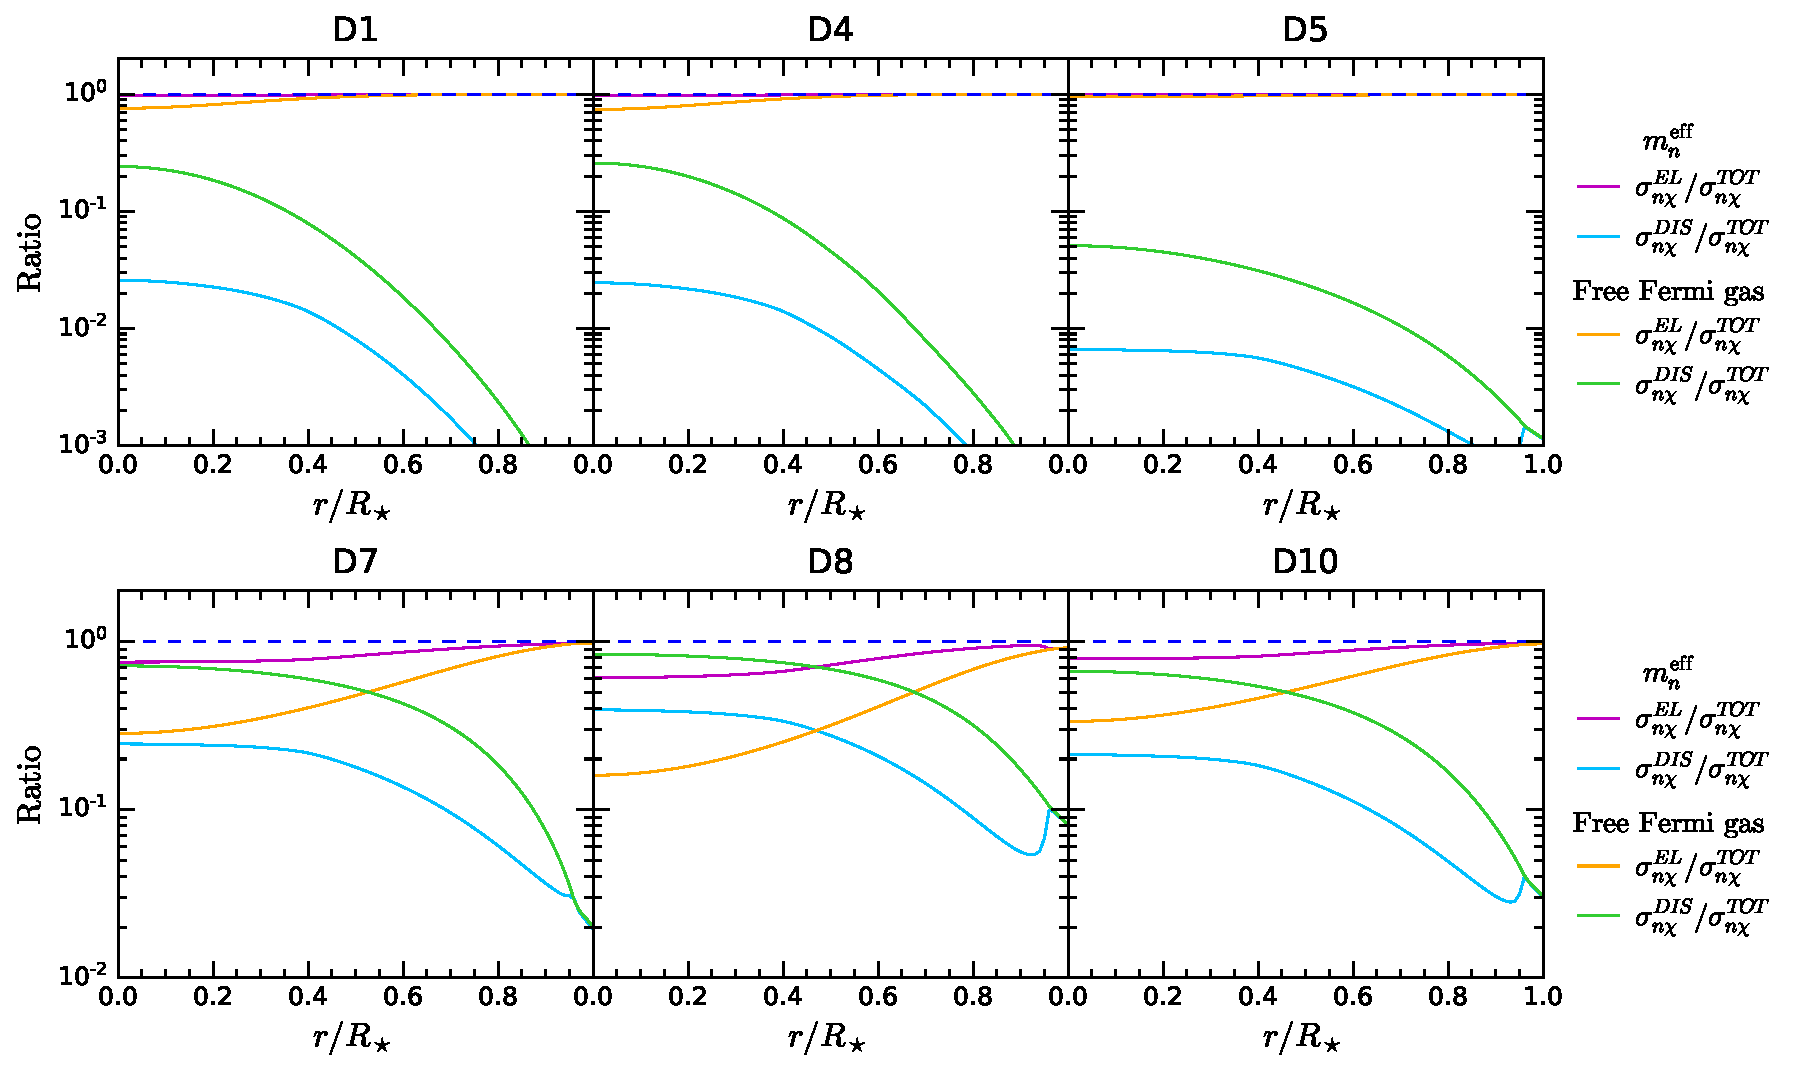
\includegraphics[width=\textwidth]{capture_3/DIS_xsectot_ratio_PeV.pdf}
    \caption{Ratios of the elastic (EL) and deep inelastic scattering (DIS) cross-sections to the total cross-section (TOT=EL+DIS) as a function of the NS radius, for neutron targets in the NS QMC-4 and six of the dimension-6 EFT operators.  We have taken $m_\chi=10^6\GeV$, and shown the comparison for both the interacting baryon and free Fermi gas approaches. Momentum-dependent form factors have been included in the elastic calculations.  }  
    \label{fig:DISratio}
\end{figure}

In addition to DIS, there may, in principle, be a contribution from the excitation of baryon resonances.  However, the resonance excitation cross-section is also expected to be suppressed. In NSs, the mass of the $\Delta$ baryon, which gives the largest contribution to this cross-section, increases with the baryon number density by between $\sim100$ and $300 \MeV$~\cite{Motta:2019ywl_Deltabaryonsplay}. This will suppress the resonance excitation cross-section significantly. Therefore, we consider only elastic collisions. 

%%%%%%%%%%%%%%%%%%%%%%%%%%%%%%%%%%%%%%%%%%%%%%%%%%%%%%%%%%%%%%%%%%%%%
%%%%%%%%%%%%%%%%%%%%%%%%%%%%%%%%%%%%%%%%%%%%%%%%%%%%%%%%%%%%%%%%%%%%%
\section{Reults from Capture on Baryons}
\label{ch5:sec:capture_results}
%%%%%%%%%%%%%%%%%%%%%%%%%%%%%%%%%%%%%%%%%%%%%%%%%%%%%%%%%%%%%%%%%%%%%
%%%%%%%%%%%%%%%%%%%%%%%%%%%%%%%%%%%%%%%%%%%%%%%%%%%%%%%%%%%%%%%%%%%%%


%%%%%%%%%%%%%%%%%%%%%%%%%%%%%%%%%%%%%%%%%%%%%%%%%%%%%%%%%%%%%%%%%%%%%
%%%%%%%%%%%%%%%%%%%%%%%%%%%%%%%%%%%%%%%%%%%%%%%%%%%%%%%%%%%%%%%%%%%%%
\section{Threshold Cross-Sections for Nucleon Scattering}
\label{ch5:sec:sigmath_results}
%%%%%%%%%%%%%%%%%%%%%%%%%%%%%%%%%%%%%%%%%%%%%%%%%%%%%%%%%%%%%%%%%%%%%
%%%%%%%%%%%%%%%%%%%%%%%%%%%%%%%%%%%%%%%%%%%%%%%%%%%%%%%%%%%%%%%%%%%%%